\documentclass{article} % For LaTeX2e
\usepackage{iclr2017_conference,times}
\usepackage{hyperref}
\usepackage{url}

\usepackage[T1]{fontenc}
\usepackage[utf8]{inputenc}
\usepackage[francais]{babel}

\usepackage{amsmath}
\usepackage{amssymb}
\usepackage{graphicx}

\title{Toward predictive machine learning for active vision}


\author{Emmanuel Daucé \\
Ecole Centrale de Marseille, Aix Marseille Univ, Inserm \\
INS, Institut de Neurosciences des Systèmes\\ 
Marseille, France\\
\texttt{emmanuel.dauce@centrale-marseille.fr} \\
}

% The \author macro works with any number of authors. There are two commands
% used to separate the names and addresses of multiple authors: \And and \AND.
%
% Using \And between authors leaves it to \LaTeX{} to determine where to break
% the lines. Using \AND forces a linebreak at that point. So, if \LaTeX{}
% puts 3 of 4 authors names on the first line, and the last on the second
% line, try using \AND instead of \And before the third author name.

\newcommand{\fix}{\marginpar{FIX}}
\newcommand{\new}{\marginpar{NEW}}

%\iclrfinalcopy % Uncomment for camera-ready version

\begin{document}


\maketitle

\begin{abstract}
Bla bla...

\end{abstract}

\section{Motivation}

	The oculo-motor activity is an essential component of man and animal behavior, subserving most of daily displacements and interactions with objects, devices or people. By moving gaze with the eyes, the center of sight is constantly and actively moving around during all waking time.  %Though taking a large part in brain activity, the principles underlying those visually guided movements are still a subject of debate in neurosciences.
	Though ubiquitous in biology, object recognition through saccades is seldom considered in artificial vision. The reasons are many, among which the existence of high-performance sensors that provide millions of pixels at low cost\footnote{on contrary to animals retina whose final design relies on a long optimization process under severe resource constraints.}. Increasingly powerful computing devices are then assigned to compute in parallel those millions of pixels to perform recognition, consuming resources in a brute-force fashion. 
	
	The example of animal vision may allow to consider computer vision differently, and possibly develop parsimonious recognition algorithms that may encompass some of its aspects. A salient aspect of animal vision is thus the use of \emph{active} sensing devices, capable of moving around under some degrees of freedom in order to choose a particular viewpoint. The existence of a set of possible sensor movements calls for the development of specific algorithms that should \emph{solve the viewpoint selection problem}. A computer vision program should for instance look back from past experience to see which viewpoint to use to provide the most useful information about a scene. Optimizing the sensor displacements across time may then be a part of computer vision algorithms, in combination with traditional pixel-based operations. 
	
	More generally, the idea of viewpoints selection turns out to consider beforehand the computations that need to be done to achieve a certain task. A virtual sensing device should for instance act like a filter that would select which part of the signal should be worth considering, and which part should be bypassed.  
	This may be the case for robots and drones  that need to react fast with light and low-power sensing devices. Similarly, in computer vision, Mega-pixel high-resolution images appeals for selective convolution over the images, in order to avoid unnecessary matrix multiplications. Less intuitively, the ever-growing  learning databases used in machine learning also suggest an intelligent scanning of the data, in a way that should retain only the critical examples or features, depending on context, before performing learning on it.  
	
	Behind the viewpoint selection problem thus lies a feature selection problem, but in that case, this feature selection heavily relies on a context. An evolving context over time implies an evolving selection of the features used in calculation. Tu put it clear, the visual features (or viewpoints) that should be used to recognize an armchair should not  be the same than the ones used to recognize a squirrel. If you are in a park, and there is a good chance to meet a squirrel, you should probably look around in the trees for something small and furry, whereas if you enter in a hotel, where there is a good chance to find an armchair, you may look sideways for something large and static, so you can ignore the "up in the tree" viewpoint and the the small and furry features, in your computations, to confirm your hypothesis.
	
	
	
	\subsection{Gaze orientation in biology}
	
	The most documented case of active perception is gaze orientation, primarily studied in both man and animal \cite{yarbus1967eye,robinson1968eye}. A nice review of principal promises of \emph{animate} vision against passive vision  is presented in \cite{ballard1991animate},  in relation with eye-hand coordination in computer vision.
	A salient feature of superior vertebrates visual apparatus is the foveated retina that concentrates  photoreceptors over a small central portion of the visual field.
	%, {\color{magenta} following an approximate exponential decrease of resolution from the center to the periphery [REF?]}. 
	 This scan of the visual scene is principally done with high-speed targeted eye movements called saccades (\cite{yarbus1967eye}), that sequentially capture local chunks of the visual scene. 
	
	\subsection{Existing work}	
	
	The concept of active vision and/or active perception is present in robotic literature under different acceptances. In \cite{aloimonos1988active}, the authors address the case of multi-view image processing of a scene, i.e. show that some ill-posed object recognition problems become well-posed problems as soon as several views on the  same object are considered. The term was also proposed in \cite{bajcsy1988active} as a roadmap for the development of artificial vision systems, that provides a first interpretation of active vision in the terms of sequential Bayesian estimation.
	
The active vision paradigm was recently introduced in neuroscience through the work of ~\cite{friston2010free,friston2012perceptions}. % 
The general setup proposed by Friston and colleagues is that of a general tendency of the brain to counteract surprising and unpredictible sensory events through building generative models that improve their predictions over time and render the world more amenable. This improvement is mainly done through sampling the environment and extracting statistical invariants that are used in return to predict upcoming events.
Building a model thus rests on extracting a repertoire of invariants and organizing them so as to process the incoming sensory data efficiently through predictive coding (see \cite{rao1999predictive}). This proposition, gathered under the ``Variational Free Energy Minimization'' umbrella, is reminiscent of the auto-encoding theory proposed by \cite{hinton1994autoencoders}, but introduces a new perspective on coding
for \emph{it formally links dictionary construction from data and (optimal) motor control}.
In particular, motor control is here considered as a particular implementation of a \emph{sampling process}, that is at the core of the estimation of a complex posterior distribution. 

The active inference approach relies on a longstanding history of probabilistic modelling in signal processing and control \cite{Kalman1960,Baum1966,friston1994statistical}.  Put formally, the physical world  takes the form of a generative process $p$ that is the cause of the sensory stream. This process is not visible in itself but is only sensed through a (non reliable) measure process that provides an observation vector $x$. The inference problem consists in estimating the underlying causes of the observation, that rests on a latent state vector $z$ and a control $u$.  Then, the evolution of $x$ relies on both $u$ and $z$ in the form of a stochastic dynamical system undergoing an external forcing command $u$, i.e. :
\begin{align}
\dot{z} &= A(z) + B(u) + \text{process noise}\label{eq:kalman-process}\\
x &= C(z) + D(u) + \text{measurement noise} \label{eq:kalman-measure}
\end{align}  
where $A$, $B$, $C$ and $D$ constitute a generative model $p(x,u,(z,\dot{z}))$ that explicits the dependencies between $u$, $x$ and $z$ \footnote{We note for simplicity $p(x,u,z)$ in the following, with each variable counting for its state vector and possible higher moments.}. 
The calculation of $\dot{z}$ from $z$ and $u$ and the calculation of $z$ from $u$ and $x$ rely on a model $p = \{A,B,C,D,\text{noise models}\}$. The model can then be inverted in order to compensate the drift of the state estimate \cite{Kalman1960,Baum1966}. The more accurate the model, the better this estimation. 

\subsection{Perception-driven control}
The question addressed by \cite{friston2012perceptions} is the design a \emph{controller} $C$ \emph{that outputs a control $u$ from $z$} so as to maximize the accuracy of this state estimation process. This is the purpose of a \emph{perception-driven} controller.

The logic behind the model is that of an external sensory scene $X$ that is never undisclosed in full, but only sensed under a particular view $x$ under sensor orientation $u$ (like it is the case in foveated vision). 
We moreover consider an organization of the visual scene in objects (or causes), whose presence and position is continuously checked by visual inspection. The objects may be described by their identity $o$ and position in space $s$, but for simplicity $o$ and $s$ are here reduced to a single variable $z = (o, s)$. 

Knowing that $z$ is invariant to changing the sensor position $u$, uncovering $z$ should rest on
collecting sensory patches $x$'s through changing $u$ (sensor orientation) across time in order to refine $z$'s estimation. 
Considering now that a certain prior $\pi(z)$ has been formed about $z$, choosing  $u$ conducts the sight in a region of the visual field that provides $x$, which in turn allows to refine the estimation of $z$.
Each saccade should consolidate a running assumption about $z$ (scene constituents), that may be retained and propagated from step to step, until enough evidence is gathered.

Instead of choosing $u$ at random, the general objective of an \emph{active inference} framework is to choose $u$ in a way that should minimize \emph{at most} the current uncertainty about $z$. 
The knowledge about $z$ can be reflected in an inference distribution $q(z)$. The better the knowledge (precision) about a sensory scene, the lower the \emph{entropy} of $q$, with:
$$H(q) = E_z[- \log q(z)]$$
It is shown in \cite{friston2012perceptions} that minimizing the entropy through action can be linked to minimizing the variational free energy attached to the sensory scene. 


%$ P(z|u,y) \propto P(y|z,u) \pi(z)$. 
%One needs thus to choose $u$ appropriately in order to reduce the uncertainty about $z$, given the actual $y$, i.e minimize the entropy :
%$u^* = \underset{u \in \mathcal{U}}{\text{argmin }} H$ with $H = E(-\log P(z|u,y))$.


The control $u$ is thus expected to reduce at most the entropy of $q(z)$ at each step. This optimal $u$ is not known in advance, because $x$ is only read \emph{after} $u$ has been carried out. Then comes the predictive framework that identifies the effect of $u$ with its most probable outcome, according to a \emph{generative} model $p$.
	
If we take a little step back, the general formulation of the generative model is that of a feedback control framework, under a discrete Bayesian inference formalism. %given a generative model $p$, and an initial condition $z_0$ (or initial guess), a control $u \in \mathcal{U}$ allows to make a \emph{prediction} about a forthcoming $z$, which allows in turn to make a prediction about the forthcoming $x$. Those 
Given an initial state $z_0$, the prediction rests on two conditional distributions, namely $p(z|u,z_0)$ --~the link dynamics that generates $z$~-- and $p(x|z,u)$ --~the measure process that generates $x$~--  (the discrete analog of (\ref{eq:kalman-process}) and (\ref{eq:kalman-measure})). %, which allows to predict the next $p(x,z|u,z_0) = p(x|z,u) p(z|u,z_0) = p(z|x,u,z_0)p(x|u,z_0)$.
Then, the forthcoming posterior distribution is (Bayes rule):
	\begin{align*}
	p(z|x,u,z_0) &= \frac{p(x,z|u,z_0)}{p(x|u,z_0)}
	= \frac{p(x|z,u) p(z|u,z_0)}{\sum_{z'}p(x|z',u) p(z'|u,z_0)}
	\end{align*}
	

	
	so that the forthcoming entropy is:
	\begin{align*}
	H(q)|_{u, z_0} &=  E_{x,z}\left[-\log  p(z|x,u,z_0)\right]
	\end{align*}
	and the optimal $u$ is:
	\begin{align*}
	\hat{u} &= \underset{u \in \mathcal{U}}{\text{argmin }} H(q)|_{u, z_0} \\
	\end{align*}
	with:
	\begin{align*}
	q(z)|_{u,z_0} &= p(z|x,u,z_0) \\
	\end{align*}
	
	In practice, the analytic calculations are out of reach (in particular for predicting the next sensory field $x$).  One thus need to consider an \emph{estimate} $\tilde{u} \simeq \hat{u}$ that should rely on sampling from the generative process $p$ to 
	predict the effect of $u$,  i.e. 
	$$ \tilde{u} = \underset{u}{\text{argmin}} \frac{1}{N} \sum_{i = 1..N, x_i \sim p, z_i \in \mathcal{Z}} -\log p(z_i| x_i, u, z_0) $$ or on an even sharper direct estimation through maximum likelihood estimates (point estimate):
	\begin{align*}
	&\tilde{u} = \underset{u}{\text{argmin }} - \log p(z_\text{max}|x_\text{max}, u, z_0)	\\
	&z_\text{max} = \underset{z}{\text{argmax }} p(z|x_\text{max}, u, z_0)\\
	&x_\text{max} = \underset{x}{\text{argmax }} p(x|u,z_0)
	\end{align*}


This operation can be repeated in a sequence, where the actual control $u = \tilde{u}$ is followed by reading the actual visual field $x$, which in turn allows to update the actual posterior distribution over $z$. This updated posterior becomes the prior of the next decision step, i.e. $z_0'\sim  p(z|x, u, z_0)$ so that a new control $u'$ can be carried out etc. 

If we denote $T$ the final step of the process,  with $u_{1:T}$ the actual sequence of controls and $x_{1:T}$ the actual sequence of observations, the final posterior estimate becomes $p(z_{1:T}|z_0, u_{1:T}, x_{1:T})$, which complies with a Hidden Markov Decision Process estimation, whose policy would be defined by the entropy minimization principles defined above, precisely to facilitate the estimation process. The active inference framework thus appears  as a \emph{state-estimation oriented policy} (it has no other purpose than facilitate estimation).

If we now turn back to the active vision analogy, $q(z_t)$ is the current assumption about the visual scene under exploration, which is used as a context ("I'm in a park with many squirrels around" --$z_t$--) to form a prediction ("If I look up, ..." --~$u_t$~-- "I may see a squirrel" --$\tilde{x}_{t+1}$--) which would reduce the entropy of the posterior $q(z_{t+1})$ for it would reduce the uncertainty about the constituents of the scene.  This incites me to look up (rather than looking down the grass) so that I can effectively process $x_{t+1}$, which may result in improving (or not) the entropy of the posterior depending whether my prediction was correct or not. I may then look to other places up around to precisely locate squirrels, but I probably don't need to inspect the grass or the lake for the same purpose, so I can currently avoid spending time looking there.   

The active perception framework allows many relieving simplification from the general POMDP estimation framework, first in considering that changing $u$ has no effect on the scene constituents, i.e. $p(z_{t+1}|u,z_t) = p(z_{t+1}|z_t)$. Then using the \emph{steady state} assumption, that considers that no significant change should take place in the scene constituents during a saccadic exploration process, i.e. $\forall t, t', z_{t} = z_{t'} = z$. This finally entails a simplified chaining of the posterior estimation:
 	\begin{align*}
 	p(z|x_{t+1},u_t) &= \frac{p(x_{t+1}|z,u_t) p(z|x_t, u_t)}{\sum_{z'}p(x_{t+1}|z',u_t) p(z'|x_t, u_t)}
 	\end{align*}
with $p(z|x_t, u_t)$ calculated at the previous step, issuing a final estimate $p(z|z_0, u_{1:T}, x_{1:T})$.  

%{\color{blue} Put in a sequential setup :
%	\begin{align*}
%	&\tilde{u}_{1:T} = \underset{u_{1:T}}{\text{argmin }} - \log p(z^\text{max}_{1:T}|x^\text{max}_{1:T}, u_{1:T}, z_0)	\\
%	&z^\text{max}_{1:T} = \underset{z_{1:T}}{\text{argmax }} p(z_{1:T}|x^\text{max}_{1:T}, u_{1:T}, z_0)\\
%	&x^\text{max}_{1:T} = \underset{x_{1:T}}{\text{argmax }} p(x_{1:T}|u_{1:T},z_0)
%	\end{align*}
%	}

\section{Implementations}

The active inference framework, that is rooted on the auto-encoding theory (Free Energy minimization) and predictive coding, provides a clear roadmap toward an effective implementation in artificial devices. It should rely on three elements, namely a generative model $p$ that should predict the next sensory scene under the current hypothesis $z$, an inference network $q$ that should predict the next posterior under putative observation $\tilde{x}$, and a policy $\rho$ that should use those predictions to issue a scene-estimation oriented control $u$.  

\begin{figure}[t!]
	\centerline{
		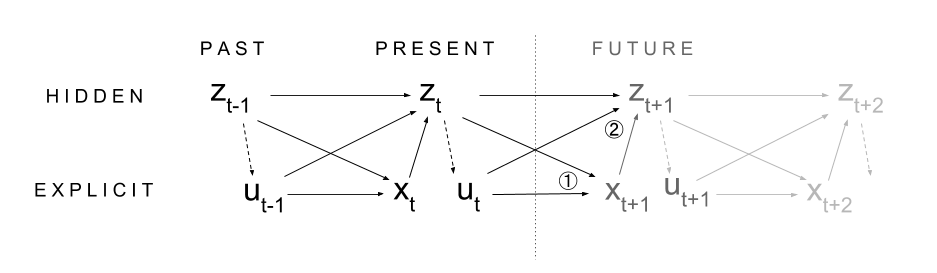
\includegraphics[width = \linewidth]{img/ICLR-graphical.png} 
	}
	\caption{Graphical model (see text)}\label{fig:graphical}
\end{figure}

Those "two-steps ahead" predictions entail a cognitive architecture based on a graphical model shown in figure \ref{fig:graphical}.
This formal similarity with usupervised auto-encoding architectures suggests that scene exploration may be learned in an unsupervised way, with both generative and predictive models learned aside to give support to the scene exploration policy. It must be noticed that the generative model (1) stems from the present $z_t$ and present $u_t$ while the inference model (2) heads toward the future $z_{t+1}$.  In the case of active vision however, we assume that $z_t = z_{t+1}$ (see previous section) so that they may be learned over the same encoding. The upper arrow represents the fact that the memory of previous state participate in the present state estimate. At least the dashed arrow represents the control policy that is not inferred but optimized from two steps ahead predictions.

Assuming the predictive and generative models are already drawn out, a \emph{model-based} approach to sequential view selection is provided in algorithm \ref{algo:saccade}. It globally complies with the predictive coding framework (\cite{rao1999predictive}) with the predictions from the actual posterior estimate used to evaluate the prediction error and update the posterior.

{\color{magenta} ALGORITHM : TODO} 

Equipped with this formalism, we can now turn to artificial vision implementation. 
A first step before a full-scale implementation is to carefully evaluate the kind of exploratory behavior provided by those principles, and see how they compare with existing active vision algorithms. 

{\color{blue}First of all, the many computer vision algorithms used to detect objects in a scene are based on highly engineered filters of low-level feature and shape extraction plus highly parallelized application of those filters over the whole image at different scales... Natural scene exploration, on contrary, uses two principal tricks to avoid unnecessary resource consumption. The first trick is the foveated retina, that concentrates the photoreceptors at the center of the retina, with a more scarce distribution at the periphery. A foveated retina allows both treating central high spatial frequencies, and peripheral low spatial frequencies at a single glance (i.e processes several scales in parallel). The second trick is the sequential saccadic scene exploration that allows to grab high spatial frequency information where it is necessary (serial processing) under some estimation oriented visuo-motor control policy. }





\subsubsection{Active perception}

The framework simplifies the general case in several ways. A first important simplification, when considering 

{\color{green} From this general standpoint, many familiar methods and principles naturally derive when considering additional details or simplifying assumptions... MODEL-BASED, SAMPLING, LEARNING (post-hoc optimization), ...}

{\color{green} from sampling $x$ from the generative process through $u$, which entail well-described form of exploration-exploitation optimization learning process [REF].}





\subsection{Visuo-motor control}

encoding distribution $q$

decoding distribution : $p$

visual orientation : $u$

visual field : $x$

\emph{steady state assumption}, i.e. $\dot{z} = 0$




In that framework, saccadic exploration means thus to define a sequence of visuo-motor commands $\tilde{u}$, $\tilde{u}'$, $\tilde{u}''$, ... This sequence should ultimately provide a final estimate $\pi^{(n)}(z)$ such that a single cause $\hat{z}$ may dominate the other ones, allowing the system to reach a final decision.  

{\color{blue}
	This can for instance be done under a greedy setup, i.e. first set $\tilde{z} = \underset{z \in \mathcal{Z}}{\text{argmax }} \pi(z)$, second set $\forall u, \tilde{y}_u = \underset{y \in \mathcal{Y}}{\text{argmax }} P(y|\tilde{z},u)$.
	Finally, set 
	\begin{equation}
	\tilde{u} = \underset{u \in \mathcal{U}}{\text{argmax }}  P(\tilde{z}|u,\tilde{y}_u))
	\end{equation} which is a proxy for minimizing the entropy. This greedy choice tells in short that if $\tilde{z}$ is the running hypothesis, the operator should orientate his sight toward 
	%the part of the scene where he thinks his assumption should receive confirmation, i.e. 
	the part of the scene that is the most discriminative toward confirming $\tilde{z}$ against all other possibilities. }
	
	
	
	
	
	{\color{blue} We show in the following that the two problems may rely on distinct processing elements in a cognitive architecture and develop (??) a probabilistic framework that may allow to address the two problems in a unified perspective. }
	
	access to the sensory signal . 
	
	i.e. Learning \emph{where to look at} then becomes the critical part, for 
	
	Our approach is not a simple XX, but may subserve important issues in the field of AI. 
	
	 seems thus to be an important field of investigation that may subserve large applicative outcomes.  
	
	%links to the case of a living system having to react at sort notice in a complex environment with limited sensors and limited computational resources. Under survival constraints and resource consuming optimization, not all the visual surroundings need to be scanned, but only the critical features, shapes and displacements. Few critical signals need to be interpreted fast, and many others can be ignored with no harm. This is the essence of visual orienting, a.k.a "active vision", that is present across most living species.  
	

	
	%The active sensing framework, that subserves  relies on emitting a signal to sense the environment, as is typically done by a radar or echolocation. Active perception  specifically considers the case of a sensing device that is moved around to increase its range and/or its resolution, where the motor displacements are there to compensate the lack of sensing capability.
	%concept of action-for-perception where a low resolution/low range  {\color{magenta} If the resulting device is significantly more complex, the global gain of sensing capabilities may be substantial.}
	\subsection{}
	
	
	
	
	The modelling of saccadic control offers thus an excellent testbed for addressing the more general active perception paradigm. It still presents many challenges, among which :
	\begin{itemize}
		\item efficiency
		\item oculomotor control and adaptation
		\item modelling and prediction
	\end{itemize}
	
	%{\color{blue} Most importantly, for efficiency reasons, the scanning of the scene through saccades needs to be sparse, i.e. select the parts of the scene.
	%Active vision needs to be encompassed in a full perception-action system view including the visual consequences of action, which emphasizes the importance of \emph{prediction} in visuomotor control \cite{Robinson1975,berthoz1996neural}} {\color{green} (attention Robinson propose un modele de prediction du mouvement lui-meme, pas des consequences visuelles du mouvement).}



\section{Model}

Papers to be submitted to ICLR 2017 must be prepared according to the
instructions presented here.

%% Please note that we have introduced automatic line number generation
%% into the style file for \LaTeXe. This is to help reviewers
%% refer to specific lines of the paper when they make their comments. Please do
%% NOT refer to these line numbers in your paper as they will be removed from the
%% style file for the final version of accepted papers.

Authors are required to use the ICLR \LaTeX{} style files obtainable at the
ICLR website. Please make sure you use the current files and
not previous versions. Tweaking the style files may be grounds for rejection.

\subsection{Retrieval of style files}

The style files for ICLR and other conference information are available on the World Wide Web at
\begin{center}
   \url{http://www.iclr.cc/}
\end{center}
The file \verb+iclr2017_conference.pdf+ contains these
instructions and illustrates the
various formatting requirements your ICLR paper must satisfy.
Submissions must be made using \LaTeX{} and the style files
\verb+iclr2017_conference.sty+ and \verb+iclr2017_conference.bst+ (to be used with \LaTeX{}2e). The file
\verb+iclr2017_conference.tex+ may be used as a ``shell'' for writing your paper. All you
have to do is replace the author, title, abstract, and text of the paper with
your own.

The formatting instructions contained in these style files are summarized in
sections \ref{gen_inst}, \ref{headings}, and \ref{others} below.

\section{General formatting instructions}
\label{gen_inst}

The text must be confined within a rectangle 5.5~inches (33~picas) wide and
9~inches (54~picas) long. The left margin is 1.5~inch (9~picas).
Use 10~point type with a vertical spacing of 11~points. Times New Roman is the
preferred typeface throughout. Paragraphs are separated by 1/2~line space,
with no indentation.

Paper title is 17~point, in small caps and left-aligned.
All pages should start at 1~inch (6~picas) from the top of the page.

Authors' names are
set in boldface, and each name is placed above its corresponding
address. The lead author's name is to be listed first, and
the co-authors' names are set to follow. Authors sharing the
same address can be on the same line.

Please pay special attention to the instructions in section \ref{others}
regarding figures, tables, acknowledgments, and references.

\section{Headings: first level}
\label{headings}

First level headings are in small caps,
flush left and in point size 12. One line space before the first level
heading and 1/2~line space after the first level heading.

\subsection{Headings: second level}

Second level headings are in small caps,
flush left and in point size 10. One line space before the second level
heading and 1/2~line space after the second level heading.

\subsubsection{Headings: third level}

Third level headings are in small caps,
flush left and in point size 10. One line space before the third level
heading and 1/2~line space after the third level heading.

\section{Citations, figures, tables, references}
\label{others}

These instructions apply to everyone, regardless of the formatter being used.

\subsection{Citations within the text}

Citations within the text should be based on the {\tt natbib} package
and include the authors' last names and year (with the ``et~al.'' construct
for more than two authors). When the authors or the publication are
included in the sentence, the citation should not be in parenthesis (as
in ``See \citet{Hinton06} for more information.''). Otherwise, the citation
should be in parenthesis (as in ``Deep learning shows promise to make progress towards AI~\citep{Bengio+chapter2007}.'').

The corresponding references are to be listed in alphabetical order of
authors, in the \textsc{References} section. As to the format of the
references themselves, any style is acceptable as long as it is used
consistently.

\subsection{Footnotes}

Indicate footnotes with a number\footnote{Sample of the first footnote} in the
text. Place the footnotes at the bottom of the page on which they appear.
Precede the footnote with a horizontal rule of 2~inches
(12~picas).\footnote{Sample of the second footnote}

\subsection{Figures}

All artwork must be neat, clean, and legible. Lines should be dark
enough for purposes of reproduction; art work should not be
hand-drawn. The figure number and caption always appear after the
figure. Place one line space before the figure caption, and one line
space after the figure. The figure caption is lower case (except for
first word and proper nouns); figures are numbered consecutively.

Make sure the figure caption does not get separated from the figure.
Leave sufficient space to avoid splitting the figure and figure caption.

You may use color figures.
However, it is best for the
figure captions and the paper body to make sense if the paper is printed
either in black/white or in color.
\begin{figure}[h]
\begin{center}
%\framebox[4.0in]{$\;$}
\fbox{\rule[-.5cm]{0cm}{4cm} \rule[-.5cm]{4cm}{0cm}}
\end{center}
\caption{Sample figure caption.}
\end{figure}

\subsection{Tables}

All tables must be centered, neat, clean and legible. Do not use hand-drawn
tables. The table number and title always appear before the table. See
Table~\ref{sample-table}.

Place one line space before the table title, one line space after the table
title, and one line space after the table. The table title must be lower case
(except for first word and proper nouns); tables are numbered consecutively.

\begin{table}[t]
\caption{Sample table title}
\label{sample-table}
\begin{center}
\begin{tabular}{ll}
\multicolumn{1}{c}{\bf PART}  &\multicolumn{1}{c}{\bf DESCRIPTION}
\\ \hline \\
Dendrite         &Input terminal \\
Axon             &Output terminal \\
Soma             &Cell body (contains cell nucleus) \\
\end{tabular}
\end{center}
\end{table}

\section{Final instructions}
Do not change any aspects of the formatting parameters in the style files.
In particular, do not modify the width or length of the rectangle the text
should fit into, and do not change font sizes (except perhaps in the
\textsc{References} section; see below). Please note that pages should be
numbered.

\section{Preparing PostScript or PDF files}

Please prepare PostScript or PDF files with paper size ``US Letter'', and
not, for example, ``A4''. The -t
letter option on dvips will produce US Letter files.

Consider directly generating PDF files using \verb+pdflatex+
(especially if you are a MiKTeX user).
PDF figures must be substituted for EPS figures, however.

Otherwise, please generate your PostScript and PDF files with the following commands:
\begin{verbatim}
dvips mypaper.dvi -t letter -Ppdf -G0 -o mypaper.ps
ps2pdf mypaper.ps mypaper.pdf
\end{verbatim}

\subsection{Margins in LaTeX}

Most of the margin problems come from figures positioned by hand using
\verb+\special+ or other commands. We suggest using the command
\verb+\includegraphics+
from the graphicx package. Always specify the figure width as a multiple of
the line width as in the example below using .eps graphics
\begin{verbatim}
   \usepackage[dvips]{graphicx} ...
   \includegraphics[width=0.8\linewidth]{myfile.eps}
\end{verbatim}
or % Apr 2009 addition
\begin{verbatim}
   \usepackage[pdftex]{graphicx} ...
   \includegraphics[width=0.8\linewidth]{myfile.pdf}
\end{verbatim}
for .pdf graphics.
See section 4.4 in the graphics bundle documentation (\url{http://www.ctan.org/tex-archive/macros/latex/required/graphics/grfguide.ps})

A number of width problems arise when LaTeX cannot properly hyphenate a
line. Please give LaTeX hyphenation hints using the \verb+\-+ command.


\subsubsection*{Acknowledgments}

Use unnumbered third level headings for the acknowledgments. All
acknowledgments, including those to funding agencies, go at the end of the paper.

\bibliography{biblio}
\bibliographystyle{iclr2017_conference}

\end{document}
